\documentclass{beamer}
\usepackage[utf8]{inputenc}

\usetheme{Madrid}
\usecolortheme{default}
\usepackage{amsmath}
\usepackage{amssymb,amsfonts,amsthm}
\usepackage{txfonts}
\usepackage{tkz-euclide}
\usepackage{listings}
\usepackage{adjustbox}
\usepackage{array}
\usepackage{tabularx}
\usepackage{gvv}
\usepackage{lmodern}
\usepackage{circuitikz}
\usepackage{tikz}
\usepackage{graphicx}

\setbeamertemplate{page number in head/foot}[totalframenumber]

\usepackage{tcolorbox}
\tcbuselibrary{minted,breakable,xparse,skins}



\definecolor{bg}{gray}{0.95}
\DeclareTCBListing{mintedbox}{O{}m!O{}}{%
  breakable=true,
  listing engine=minted,
  listing only,
  minted language=#2,
  minted style=default,
  minted options={%
    linenos,
    gobble=0,
    breaklines=true,
    breakafter=,,
    fontsize=\small,
    numbersep=8pt,
    #1},
  boxsep=0pt,
  left skip=0pt,
  right skip=0pt,
  left=25pt,
  right=0pt,
  top=3pt,
  bottom=3pt,
  arc=5pt,
  leftrule=0pt,
  rightrule=0pt,
  bottomrule=2pt,
  toprule=2pt,
  colback=bg,
  colframe=orange!70,
  enhanced,
  overlay={%
    \begin{tcbclipinterior}
    \fill[orange!20!white] (frame.south west) rectangle ([xshift=20pt]frame.north west);
    \end{tcbclipinterior}},
  #3,
}
\lstset{
    language=C,
    basicstyle=\ttfamily\small,
    keywordstyle=\color{blue},
    stringstyle=\color{orange},
    commentstyle=\color{green!60!black},
    numbers=left,
    numberstyle=\tiny\color{gray},
    breaklines=true,
    showstringspaces=false,
}
\title{1.5.33}
\date{21st August, 2025}
\author{Puni Aditya - EE25BTECH11046}

\begin{document}

\frame{\titlepage}
\begin{frame}{Question}
Find the ratio in which the Y-axis divides the line segment joining the points A\brak{5, -6} and B\brak{-1, -4}. Also find the coordinates of the point of intersection.
\end{frame}

\begin{frame}{allowframebreaks}
\frametitle{Equation}
Let the Y-axis divide the line segment $\vec{AB}$ at point $\vec{P}$ in the ratio $k:1$.
Since $\vec{P}$ lies on Y-axis, let
\begin{align*}
\vec{P} = \myvec{0 \\ y}
\end{align*}
The point $\vec{A}$, $\vec{B}$, $\vec{P}$ are collinear.
\begin{align}
\implies \text{rank}\myvec{\vec{B}-\vec{A} & \vec{P}-\vec{A}} = 1
\end{align}
\end{frame}

\begin{frame}[fragile]
	\frametitle{Theoretical Solution}
\begin{align}
	\myvec{-6 & -5 \\ 2 & y+6} \xleftrightarrow[]{R_2 \rightarrow {\frac{1}{3}R_1 + R_2}} \myvec{-6 & -5 \\ 0 & y+\frac{13}{3}}  
\end{align}
The number of nonzero rows in the row reduced matrix (also known as {\em echelon form}) is defined as the rank. For above matrix to be of rank 1,
\begin{align}
y+\frac{13}{3} &= 0 \\
y &= \frac{-13}{3}
\end{align}
$\therefore$ The coordinates of the point of intersection are 
\begin{align*}
\vec{P} = \myvec{0 \\ \frac{-13}{3}}
\end{align*}
\end{frame}

\begin{frame}{allowframebreaks}
\frametitle{Theoretical Solution}
Substituting the values of $\vec{A}$, $\vec{B}$ and $\vec{P}$,
\begin{align}
k=\frac{\myvec{5 & \frac{-5}{3}}\myvec{1 \\ \frac{-1}{3}}}{\norm{\myvec{1 \\ \frac{-1}{3}}}^2}=5
\end{align}

Thus, the ratio in which the point $\vec{P}$ divides the line segment $\vec{AB}$ is \textbf{5:1}.
\end{frame}

\begin{frame}[fragile]
    \frametitle{C Code}
    \begin{lstlisting}
#include <stdio.h>
#include <math.h>
void function(double *P, double *B, double *A , int m, int k) {
    for ( int i = 0 ; i < m ; i++ ) {
        P[i] = (1*A[i] + k*B[i])/(k+1) ; 
    }
}
    \end{lstlisting}
\end{frame}

\begin{frame}[fragile]
    \frametitle{Python Code}
    \begin{lstlisting}
import sys
import math
import numpy as np
import matplotlib.pyplot as plt
import ctypes

section_formula = ctypes.CDLL('/home/puniaditya/GitHub/ee1030-2025/ee25btech11046/matgeo/1.5.33/codes/section_formula.so')
    \end{lstlisting}
\end{frame}

\begin{frame}[fragile]
    \frametitle{Python Code}
    \begin{lstlisting}
section_formula.argtypes = [
    ctypes.POINTER(ctypes.c_double),
    ctypes.POINTER(ctypes.c_double),
    ctypes.POINTER(ctypes.c_double),
    ctypes.c_int,
    ctypes.c_int,
]
section_formula.restype = None  # void function

m = 2
k = 5

A = np.array([[5, -6]], dtype=np.float64)
B = np.array([[-1, -4]], dtype=np.float64)
P = np.zeros(m, dtype=np.float64)
    \end{lstlisting}
\end{frame}

\begin{frame}[fragile]
    \frametitle{Python Code}
    \begin{lstlisting}
section_formula.function(
    P.ctypes.data_as(ctypes.POINTER(ctypes.c_double)),
    B.ctypes.data_as(ctypes.POINTER(ctypes.c_double)),
    A.ctypes.data_as(ctypes.POINTER(ctypes.c_double)),
    m, #len(P) alternate
    k
)

A = np.array([5, -6]).reshape(-1,1)
B = np.array([-1, -4]).reshape(-1,1)
P = P.reshape(-1,1)
    \end{lstlisting}
\end{frame}

\begin{frame}[fragile]
    \frametitle{Python Code}
    \begin{lstlisting}
plt.plot([A[0,0], B[0,0]], [A[1,0], B[1,0]], 'g--', label="Line Segment AB")

plot_coords = np.block([[A, B, P]])
plt.scatter(plot_coords[0,:], plot_coords[1,:], color='blue')

vert_labels = [
    f'A({A[0,0]}, {A[1,0]})',
    f'B({B[0,0]}, {B[1,0]})',
    f'P({P[0,0]}, {P[1,0]:.2f})'
]
    \end{lstlisting}
\end{frame}

\begin{frame}[fragile]
    \frametitle{Python Code}
    \begin{lstlisting}
for i, txt in enumerate(vert_labels):
    plt.annotate(txt,
            (plot_coords[0,i],plot_coords[1,i]),
            textcoords="offset points",
            xytext=(0,10),
            ha='center')

plt.xlabel('$x$')
plt.ylabel('$y$')
plt.title("Line Segment AB Divided by Y-axis")
plt.legend(loc='best')
plt.grid()
plt.axis('equal')

plt.savefig("../figs/plot_c.jpg")
plt.show()
    \end{lstlisting}
\end{frame}

\begin{frame}{Plot}
    \begin{figure}
        \centering
        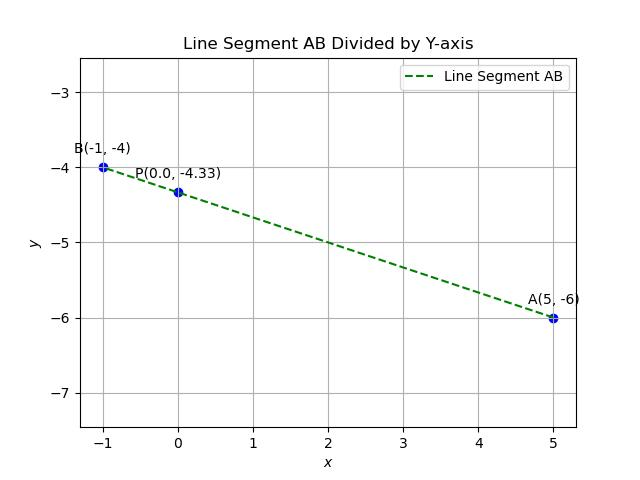
\includegraphics[width=0.5\columnwidth]{../figs/plot_c.jpg}
        \caption{Plot of Intersection of AB by Y-axis}
        \label{fig:fig}
    \end{figure}
\end{frame}




\end{document}
